\documentclass{standalone}
\usepackage{tikz}
\begin{document}
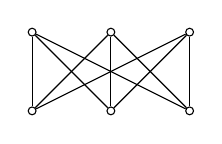
\begin{tikzpicture}[every node/.style={circle, inner sep=1pt, draw=black}]
  \foreach \n in {1, 2, 3}{
    \pgfmathsetmacro{\x}{\n - 2}

    \node (t\n) at (\x,  .5) {};
    \node (b\n) at (\x, -.5) {};
  }

  \foreach \n in {1,2,3}{
    \foreach \m in {1,...,3}{
      \draw (t\n) -- (b\m);
    }
  }

\end{tikzpicture}
\end{document}
